\documentclass[a4j,12pt,]{jarticle}
 \usepackage[dvipdfmx]{graphicx}
 \usepackage{float}
 \usepackage{siunitx} %%SI単位系用
 \usepackage{amssymb, amsmath}
 \usepackage{ascmac,here,txfonts,txfonts}
\usepackage{listings,jlisting}
\usepackage[dvipdfmx]{color}
\lstset{%
  language={Python},
  basicstyle={\small},%
  identifierstyle={\small},%
  commentstyle={\small\itshape\color[rgb]{0,0.5,0}},%
  keywordstyle={\small\bfseries\color[rgb]{0,0,1}},%
  ndkeywordstyle={\small},%
  stringstyle={\small\ttfamily\color[rgb]{1,0,1}},
  frame={tb},
  breaklines=true,
  columns=[l]{fullflexible},%
  numbers=left,%
  xrightmargin=0zw,%
  xleftmargin=3zw,%
  numberstyle={\scriptsize},%
  stepnumber=1,
  numbersep=1zw,%
  lineskip=-0.5ex%
}
\begin{document}

{\noindent\small 第17回報告書 \hfill\today}
\begin{center}
  {\Large 分布定数線路の周波数特性}
\end{center}
\begin{flushright}
  愛媛大学工学部 \\
  8531037m \\
  祖父江匠真 \\
\end{flushright}

\section{はじめに}

今回は, ケーブルをマッチング, もしくはマッチングせず受電端側を短絡, 開放した回路における周波数特性, 共振, 反共振について, また入力波形として方形波を入力した際の出力波形について調べたので報告する.

\section{分布定数線路の周波数特性}

伝達関数の計算には, 図\ref{p1}に分布定数線路のF行列

\large
\[
  \left(
  \begin{array}{cc}
      A & B \\
      C & D
    \end{array}
  \right) =
  \left(
  \begin{array}{cc}
      \cosh\gamma l             & Z_0\sinh\gamma l \\
      \frac{\sinh\gamma l}{Z_0} & \cosh\gamma l
    \end{array}
  \right)
\]
\normalsize

と, $R_1 = 0$[Ω]を代入して求めた

\large
\begin{eqnarray}
  G(f) =  \frac{1}{\cosh\gamma l + \frac{Z_0\sinh\gamma l}{R_2}}
\end{eqnarray}
\normalsize

を使用した.

また, $R_2$は, 無損失ケーブルについては, マッチングした場合, マッチングせず受電端側を短絡した場合, 開放した場合でそれぞれ, 50[Ω], 0[Ω], $1.0 × 10^{6}$[Ω]とし, ケーブルの特性インピーダンスは$Z_0 = 50(Ω)$として計算した.

$\gamma$ は
\begin{eqnarray}
  \gamma =  \sqrt{(R + j\omega L)(G + j\omega C)}
\end{eqnarray}
から求めた.
$\gamma$を計算する際の回路素子の値について, Cの値はC = $1.0 × 10^{-10}$[F/m]とし, Lは特性インピーダンス$Z_0$とCを用いて

\large
\begin{eqnarray}
  Z_0 =  \sqrt{\frac{L}{C}}
\end{eqnarray}
\normalsize

より, L = $2.5 × 10^{-7}$ [H/m]とした.

また, R, Gについては無損失ケーブルは, R = 0 [Ω/m], G = 0 [S/m], 損失有りのケーブルでは, R = $1.0 × 10^{-3}$[Ω/m]とし, R = $1.0 × 10^{-4}$[S/m] ケーブル長である$l$は, $l = 1000$[m]として計算した.

\begin{figure}[H]
  \begin{center}
    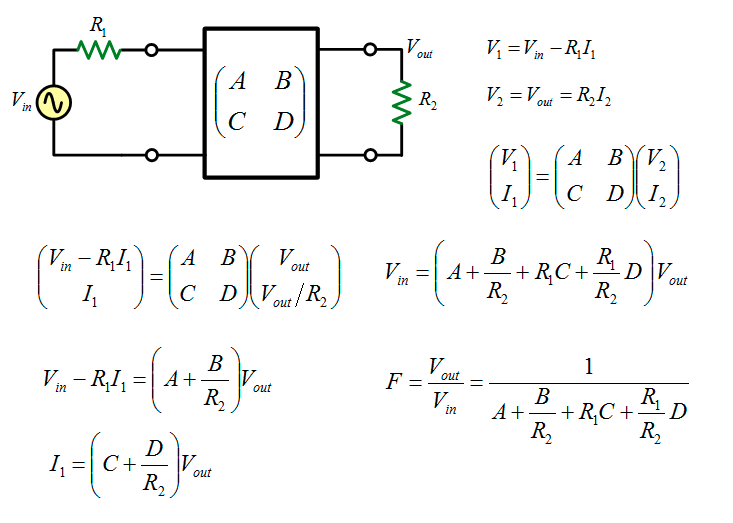
\includegraphics[width=140mm]{transfer.png}
    \caption{F行列から伝達関数を導出する過程}
    \label{p1}
  \end{center}
\end{figure}

以上の条件において, 無損失ケーブルをマッチング, もしくはマッチングせず受電端側を短絡, 開放した場合に求めた周波数特性を図\ref{p2}, \ref{p3}, \ref{p4}に示す.

また, 受電端短絡における共振周波数, 反共振周波数をそれぞれ

\begin{eqnarray}
  f =  \frac{n}{2l\sqrt{LC}}\;\;\;\;\;(n = 1, 2, ...)
\end{eqnarray}

\begin{eqnarray}
  f =  \frac{2n + 1}{4l\sqrt{LC}}\;\;\;\;\;(n = 0, 1, 2, ...)
\end{eqnarray}

受電端開放における共振周波数, 反共振周波数をそれぞれ

\begin{eqnarray}
  f =  \frac{2n + 1}{4l\sqrt{LC}}\;\;\;\;\;(n = 0, 1, 2, ...)
\end{eqnarray}

\begin{eqnarray}
  f =  \frac{n}{2l\sqrt{LC}}\;\;\;\;\;(n = 1, 2, ...)
\end{eqnarray}

により求め図\ref{p3}, \ref{p4}にプロットしている.

\begin{figure}[H]
  \begin{center}
    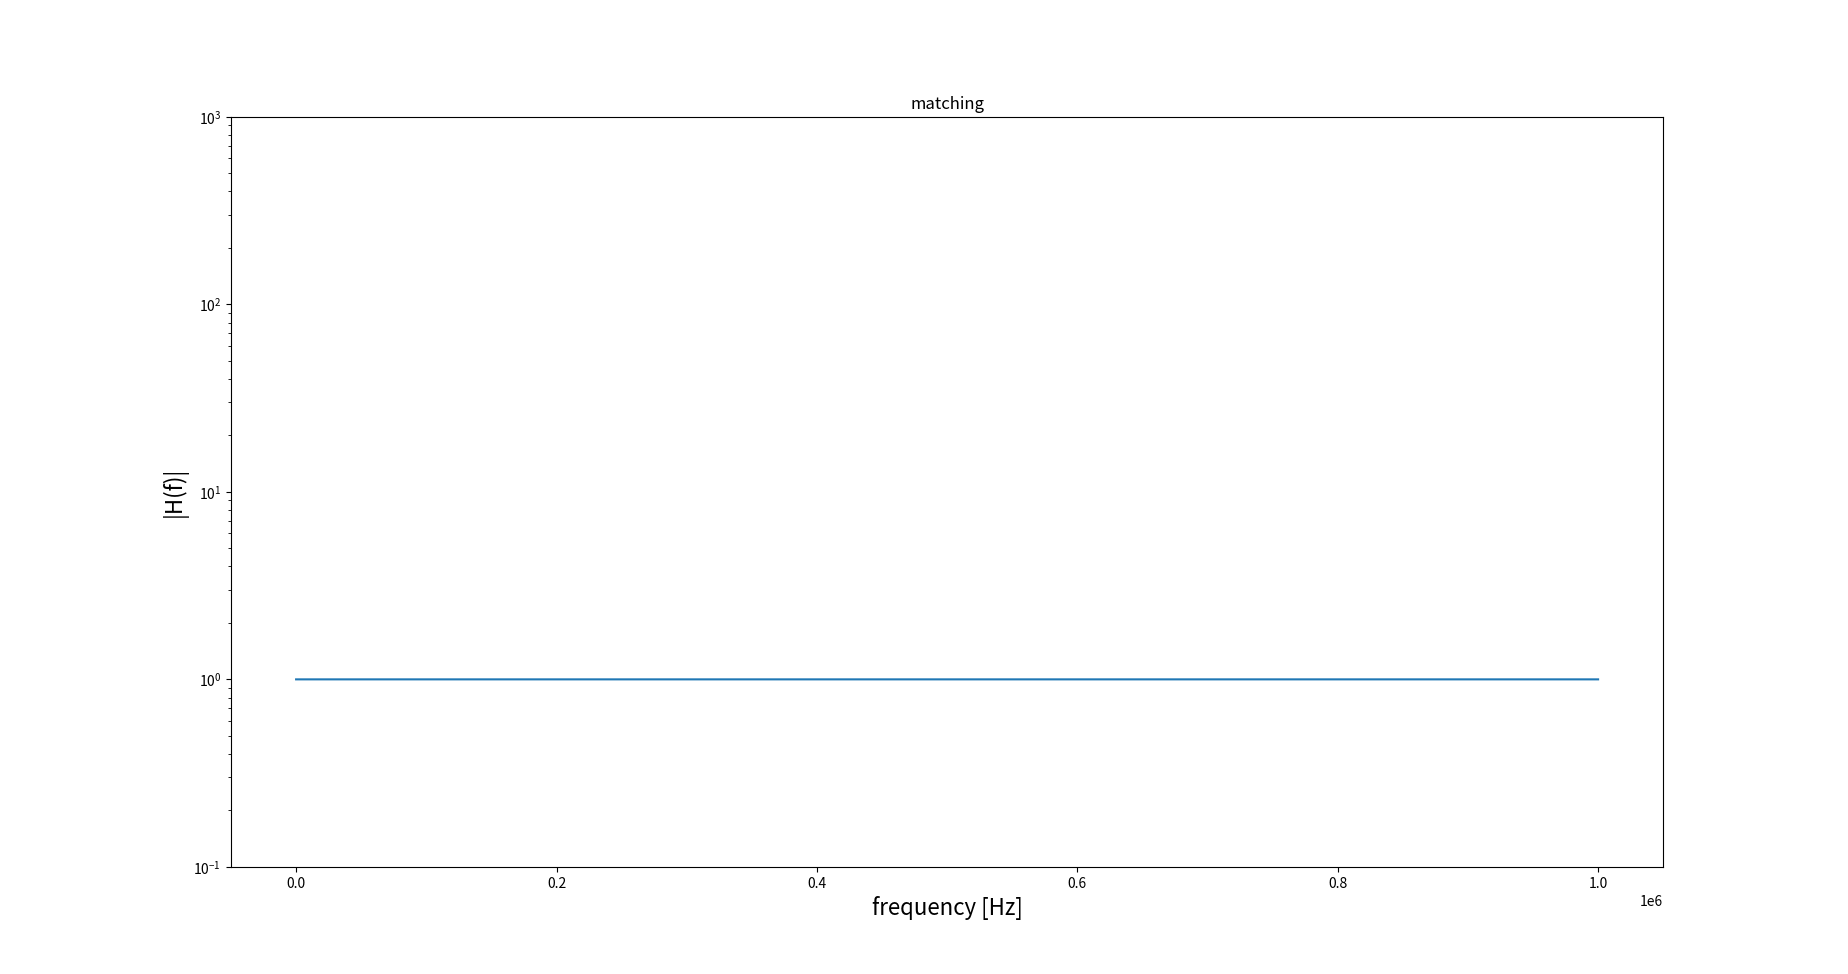
\includegraphics[width=160mm]{report/matchingWithoutDampingConstantsLogScale.png}
    \caption{マッチングした場合における周波数特性}
    \label{p2}
  \end{center}
\end{figure}

\begin{figure}[H]
  \begin{center}
    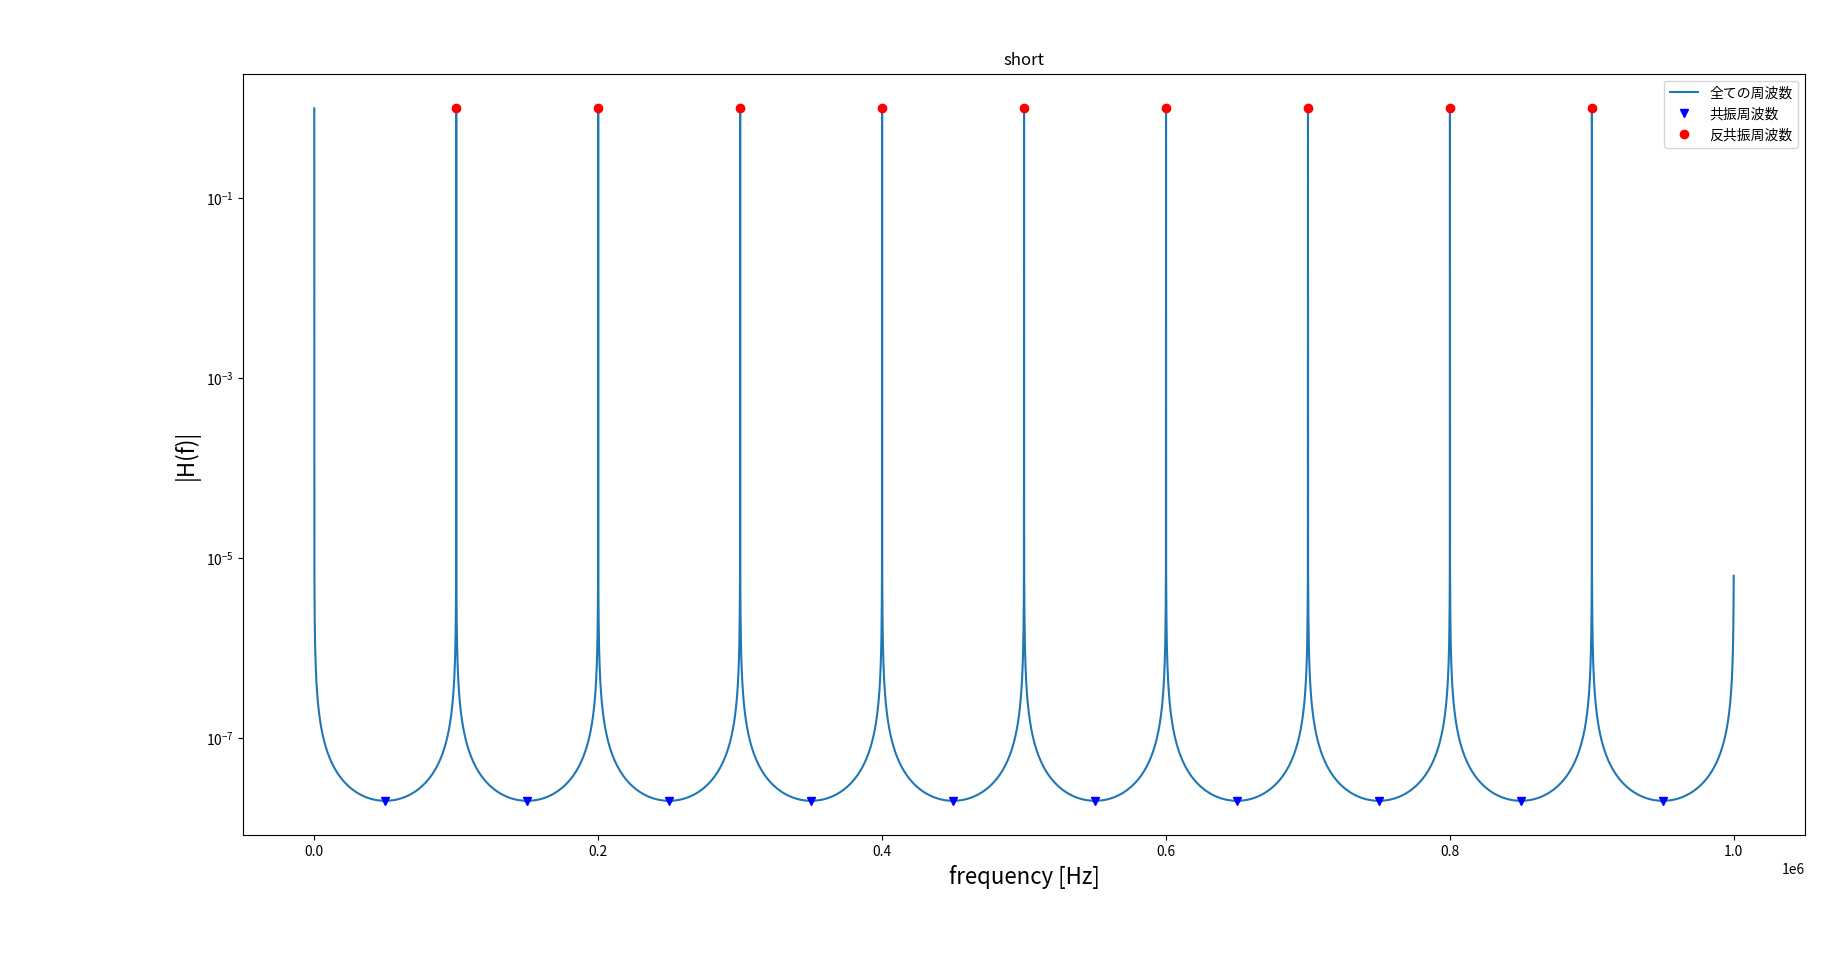
\includegraphics[width=160mm]{report/shortCircuitAtReceivingEndWithoutDecayConstantLogScale.png}
    \caption{マッチングせず受電端側を短絡した場合における周波数特性}
    \label{p3}
  \end{center}
\end{figure}

\begin{figure}[H]
  \begin{center}
    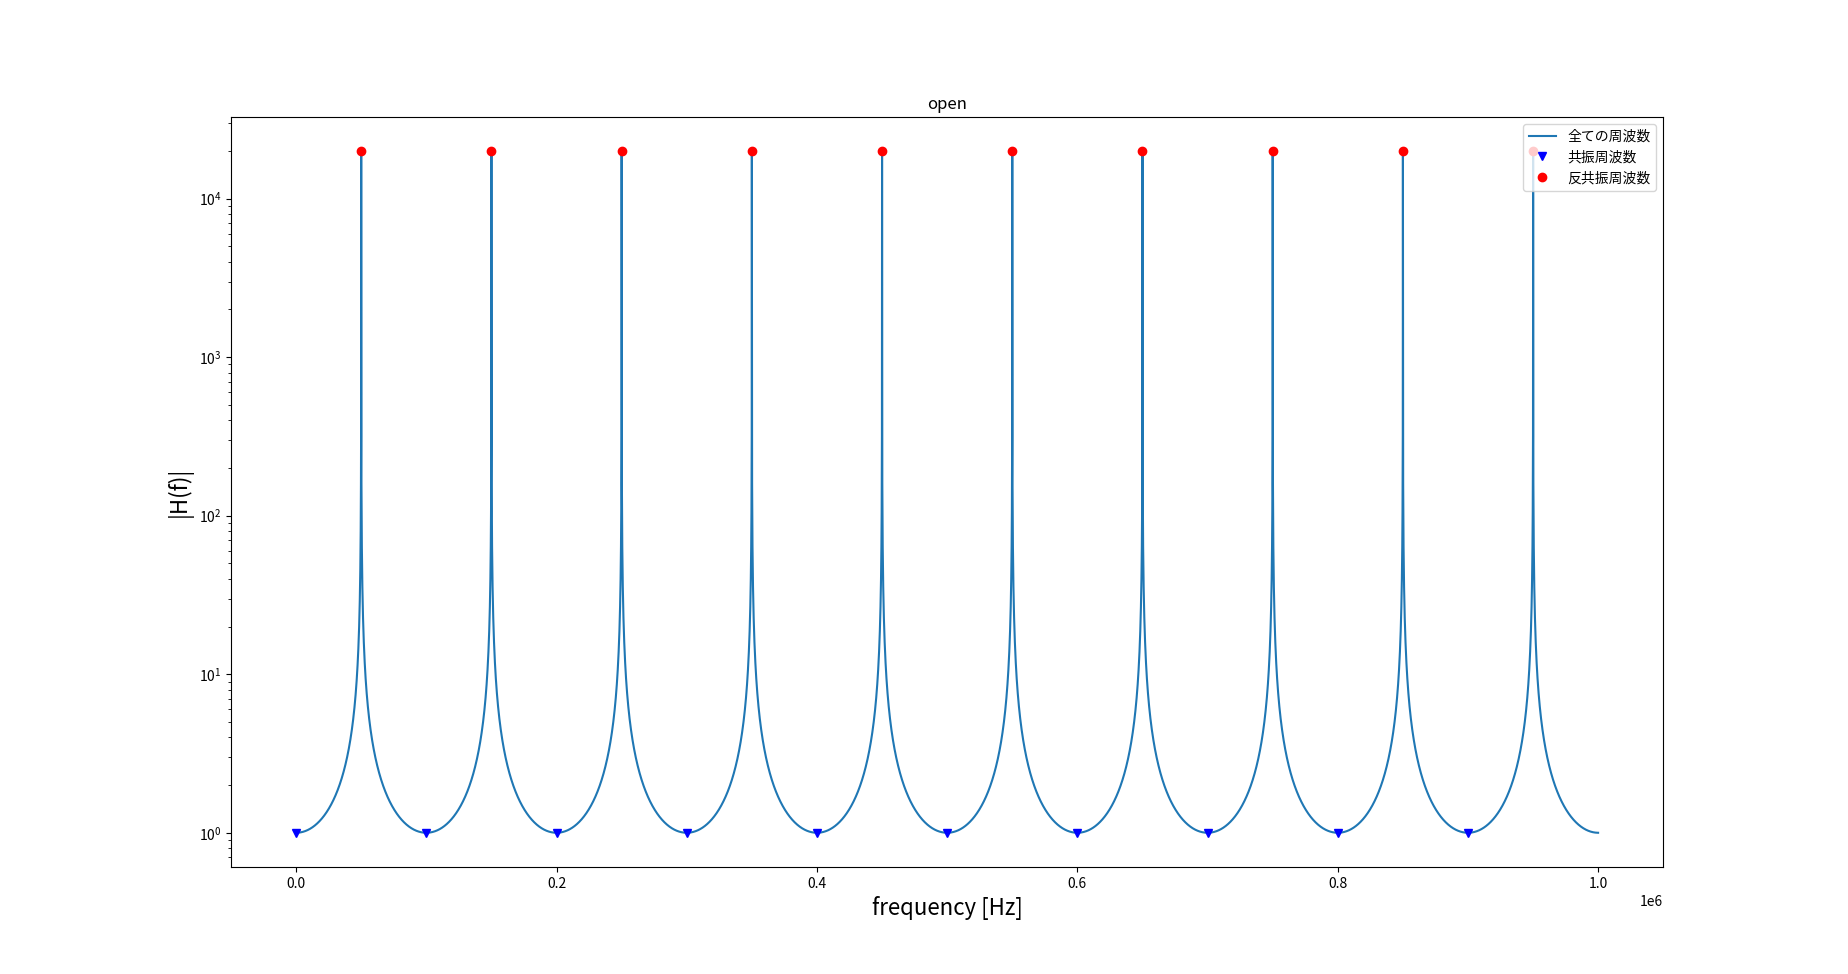
\includegraphics[width=160mm]{report/receivingEndOpenWithoutAttenuationConstantLogScale.png}
    \caption{マッチングせず受電端側を開放した場合における周波数特性}
    \label{p4}
  \end{center}
\end{figure}

次に, 損失有りのケーブルを受電端側を短絡, 開放した場合に求めた周波数特性を図\ref{p5}, \ref{p6}に示す.

\begin{figure}[H]
  \begin{center}
    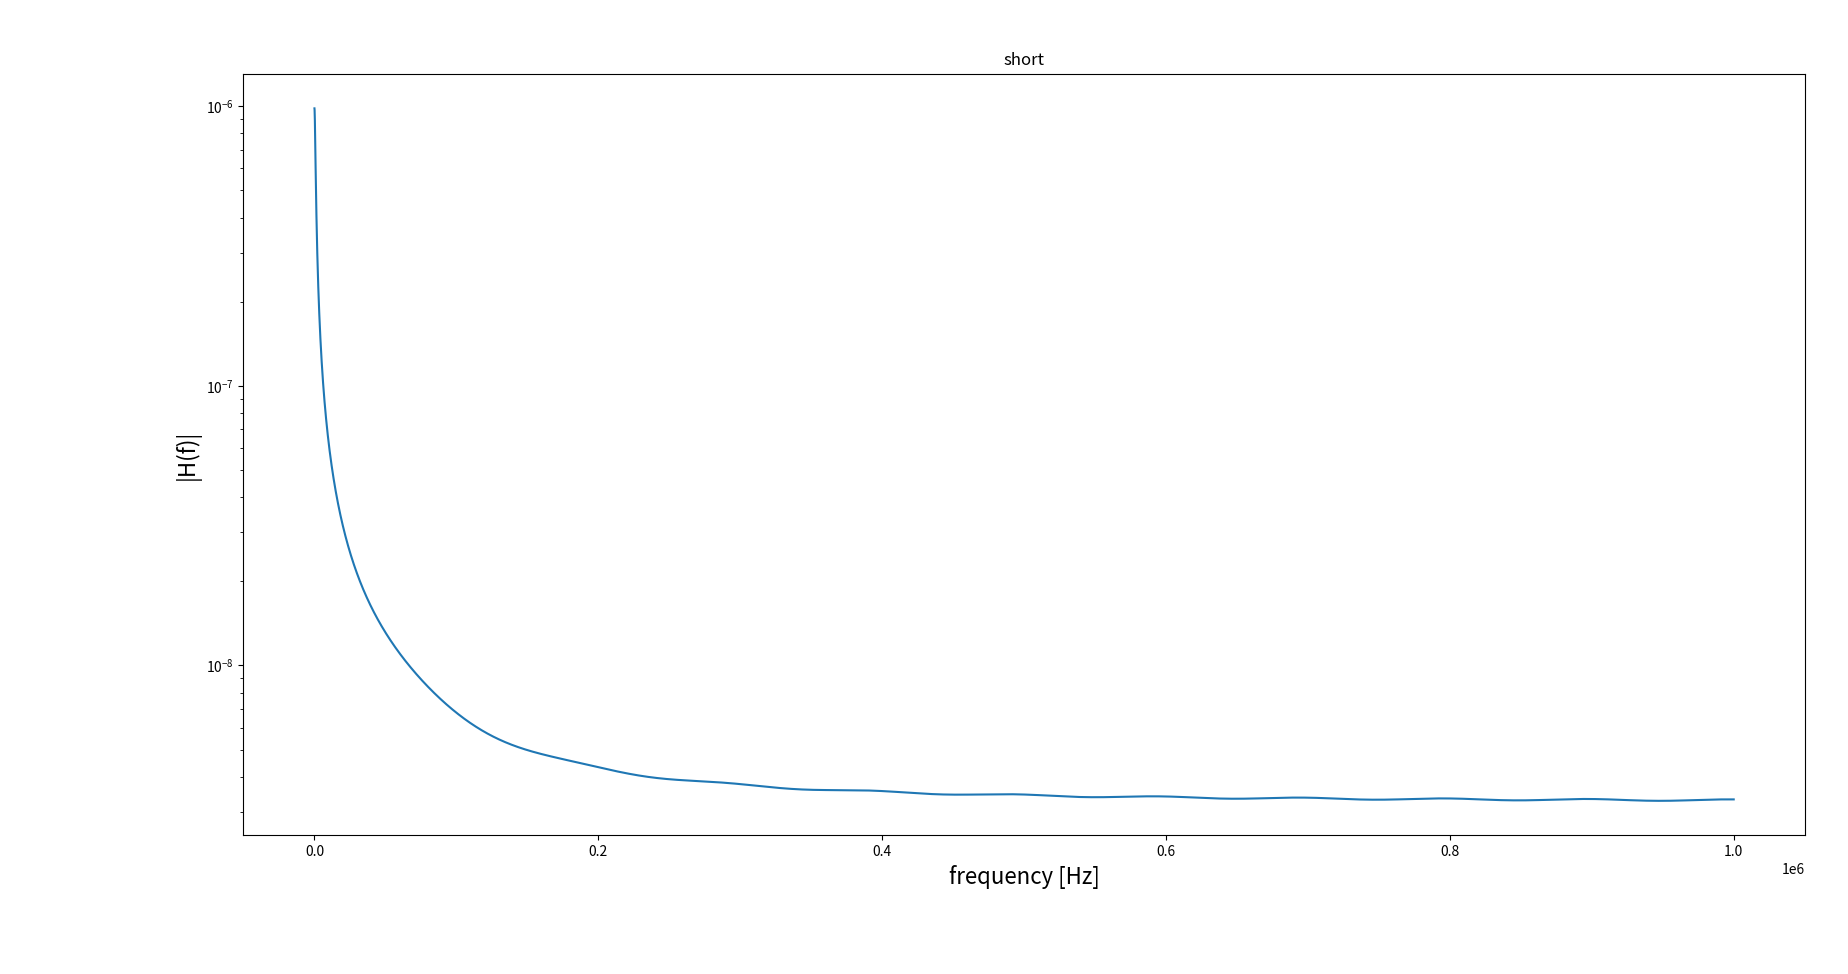
\includegraphics[width=160mm]{report/shortCircuitAtReceivingEndWithDampingConstantLogScale.png}
    \caption{受電端側を短絡した場合における周波数特性}
    \label{p5}
  \end{center}
\end{figure}

\begin{figure}[H]
  \begin{center}
    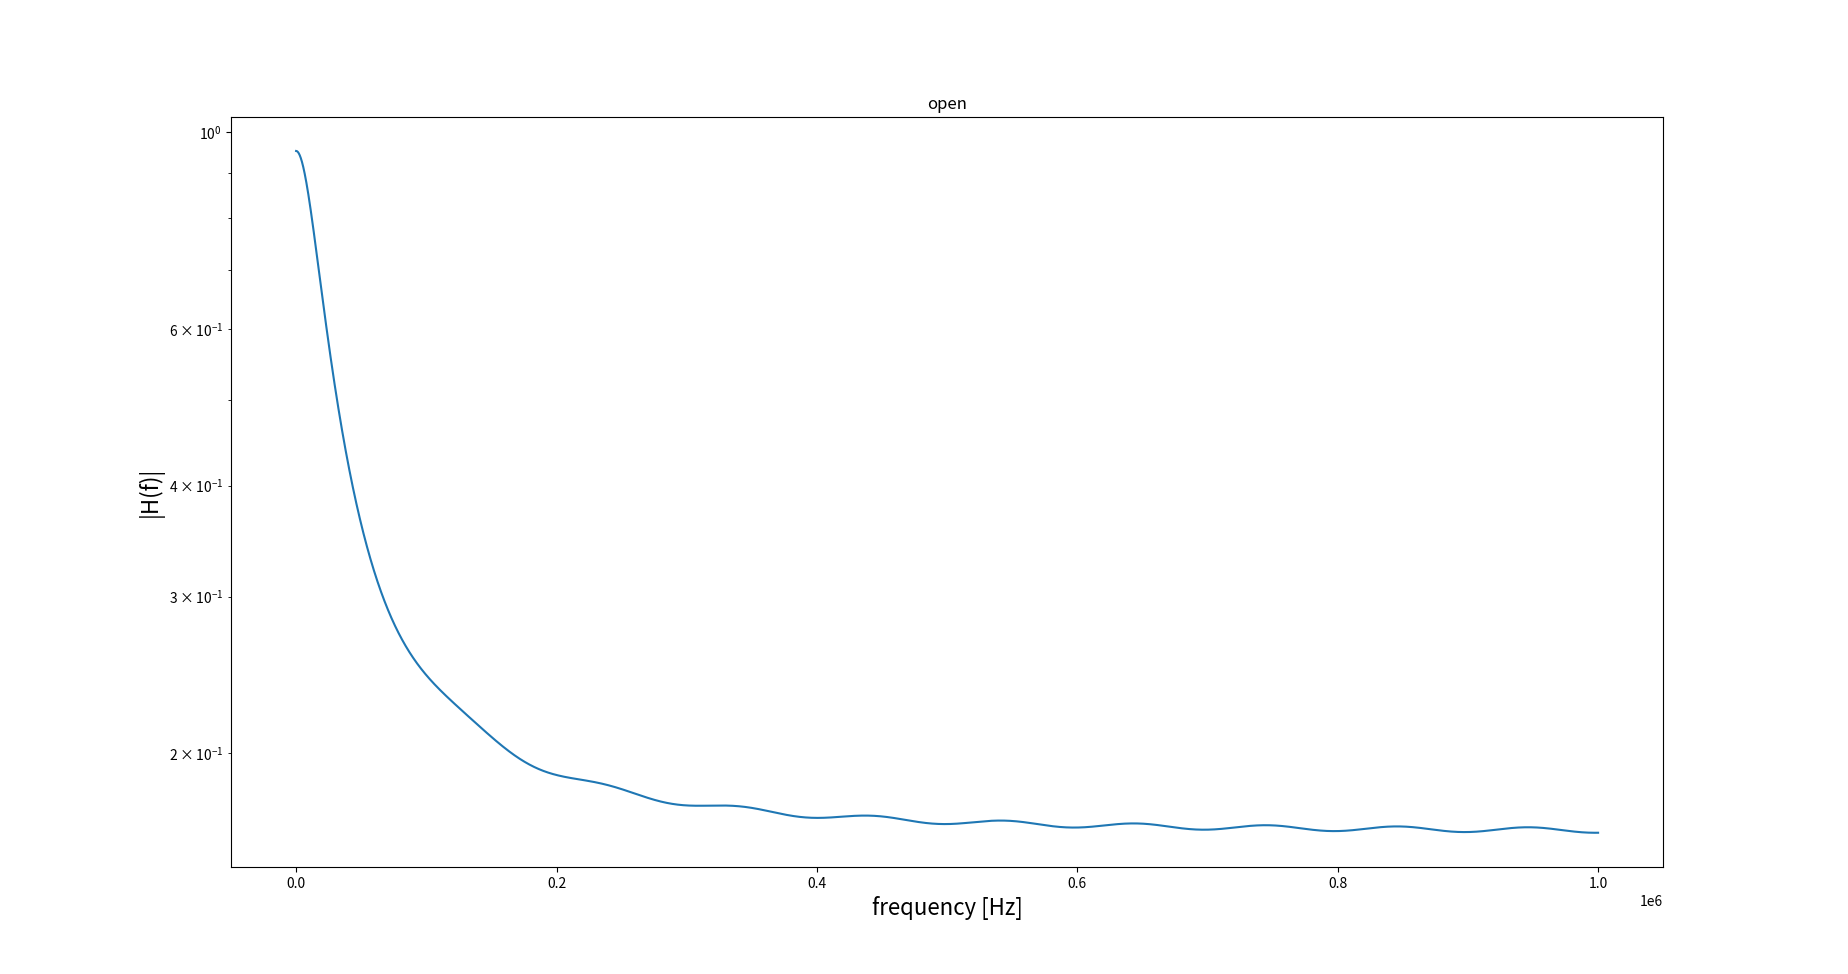
\includegraphics[width=160mm]{report/openAtReceivingEndWithAttenuationConstantLogScale.png}
    \caption{受電端側を開放した場合における周波数特性}
    \label{p6}
  \end{center}
\end{figure}

次に, 受電端を短絡, 開放した損失有りのケーブルに, 方形波を入力した際の出力波形について報告する.

入力波形を図\ref{p7}, 入力波形をフーリエ変換したものを図\ref{p8}に示す.

\begin{figure}[H]
  \begin{center}
    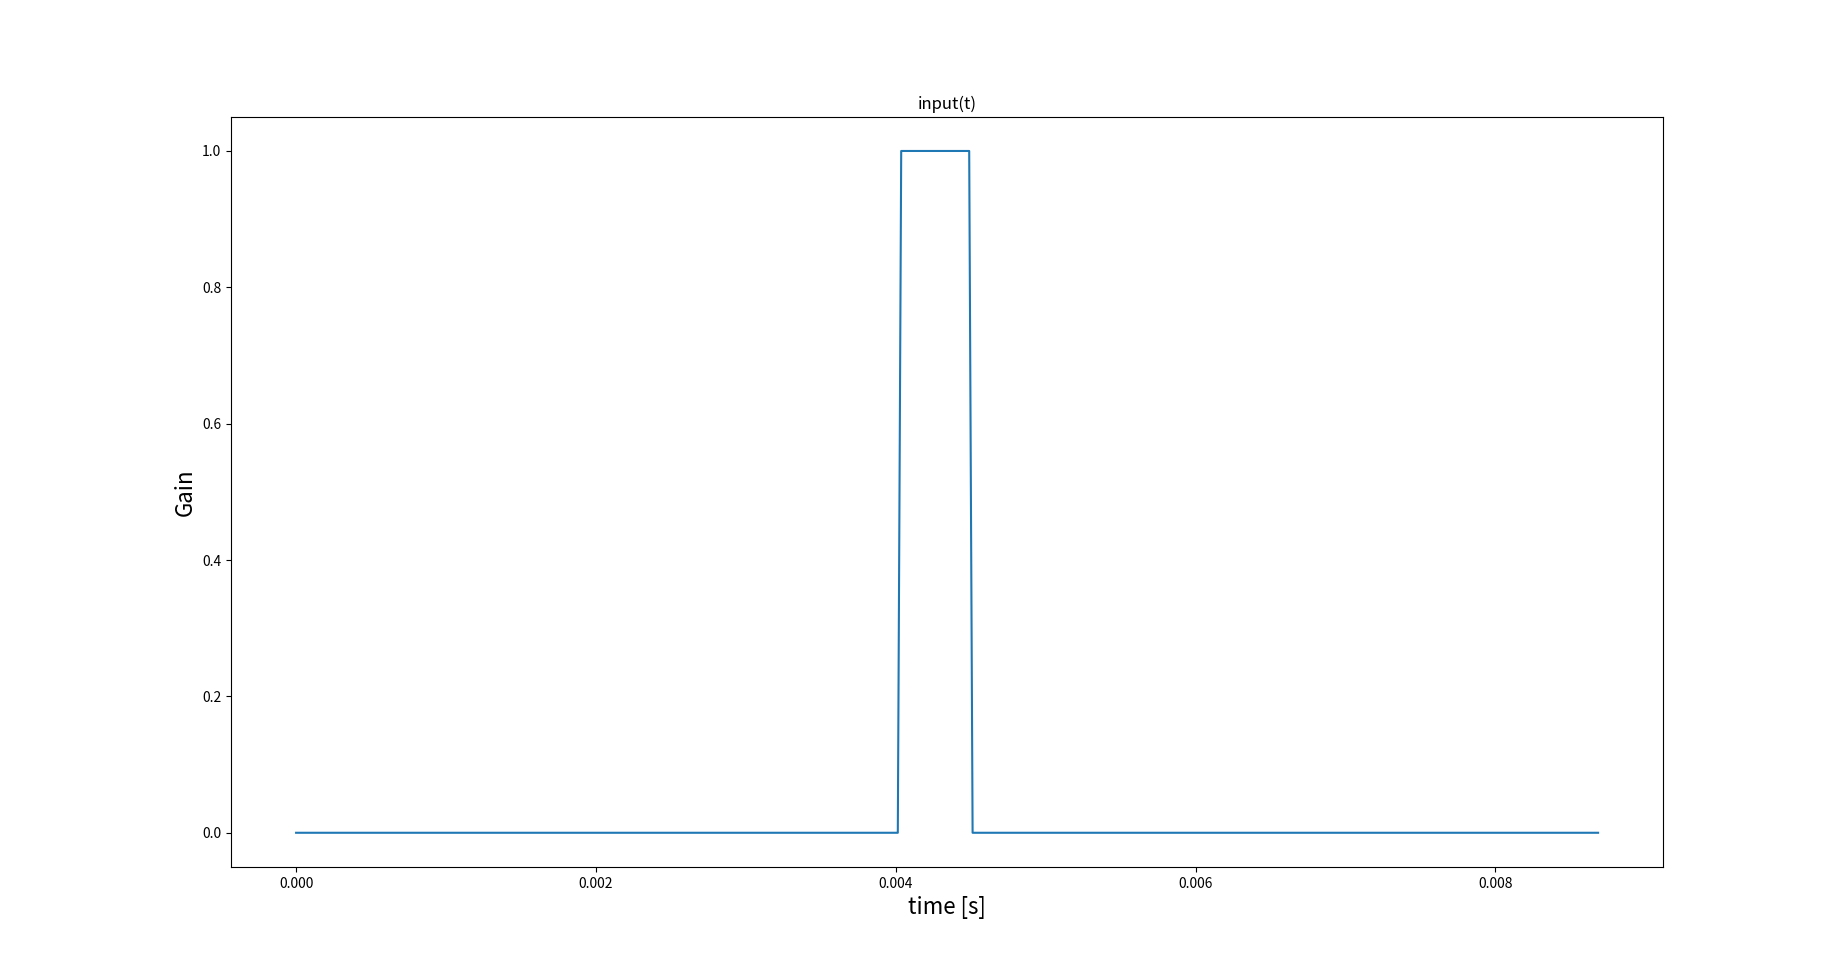
\includegraphics[width=160mm]{report/inputWaveformTimeAxis.png}
    \caption{入力波形}
    \label{p7}
  \end{center}
\end{figure}

\begin{figure}[H]
  \begin{center}
    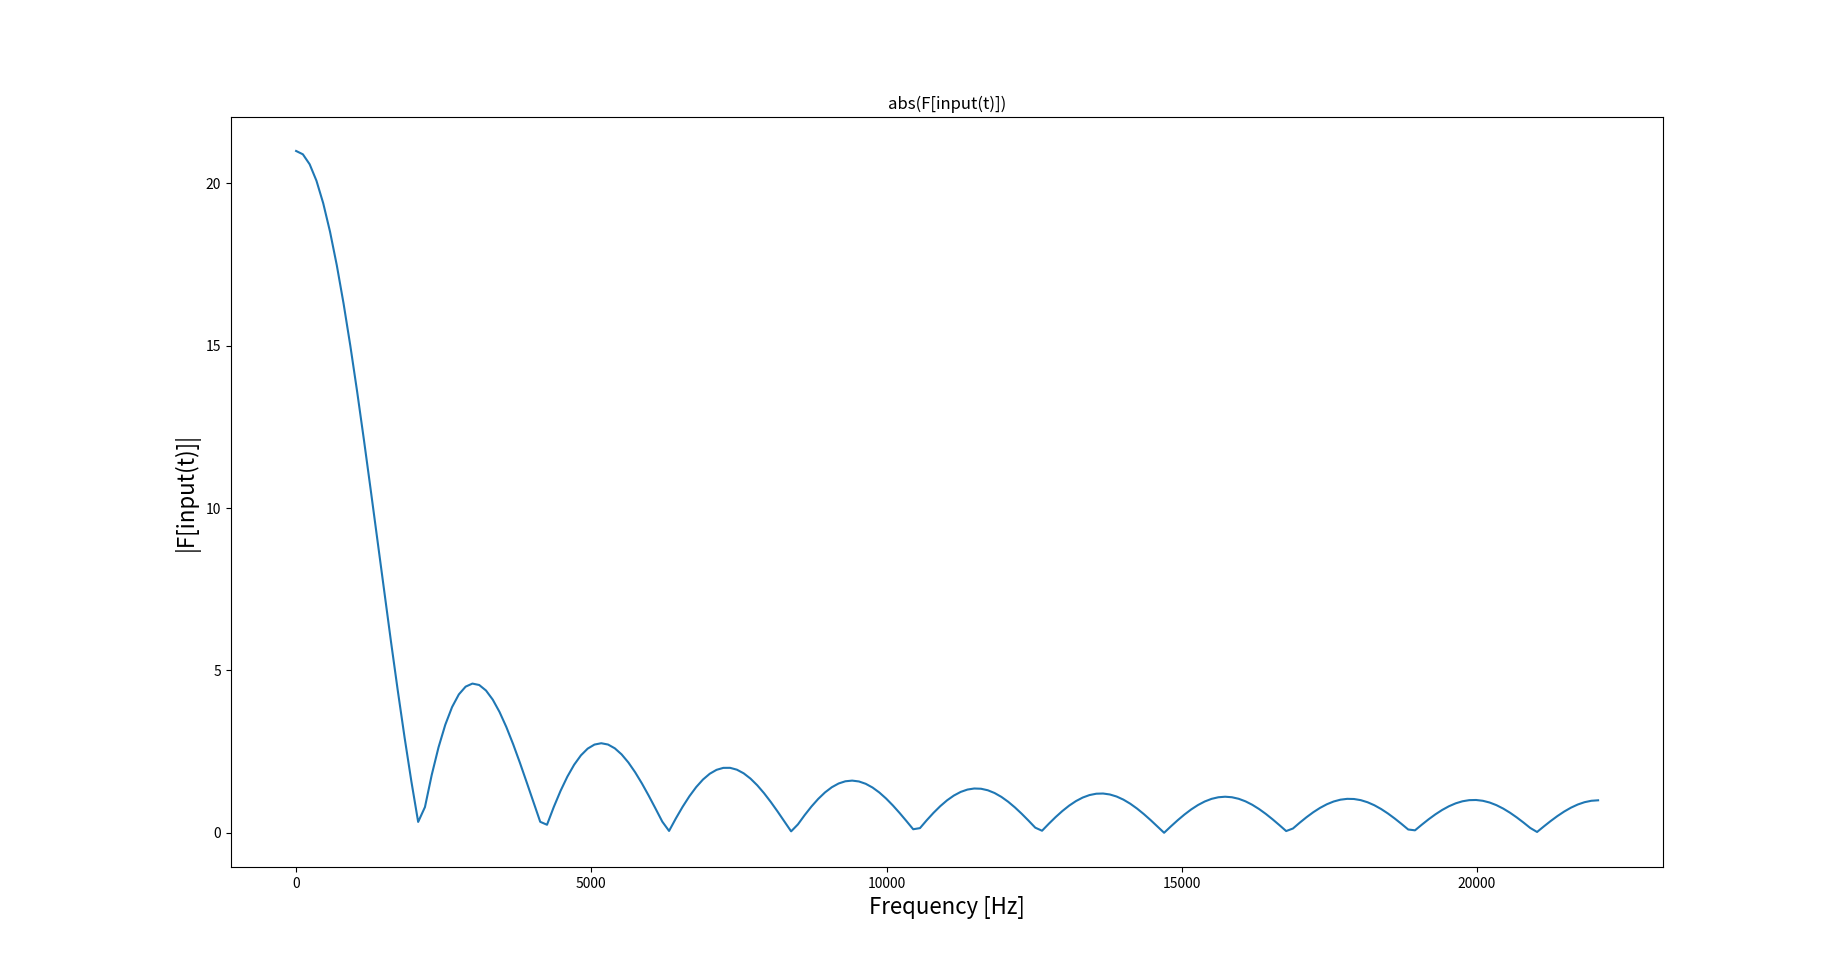
\includegraphics[width=160mm]{report/inputWaveformFFT.png}
    \caption{入力波形をフーリエ変換したもの}
    \label{p8}
  \end{center}
\end{figure}

受電端を短絡した場合の伝達関数, 伝達関数と入力波形をフーリエ変換したものの積, 伝達関数と入力波形をフーリエ変換したものの積を逆フーリエ変換して時間軸に戻した出力波形をそれぞれ図\ref{p9}, \ref{p10}, \ref{p11}に示す.

\begin{figure}[H]
  \begin{center}
    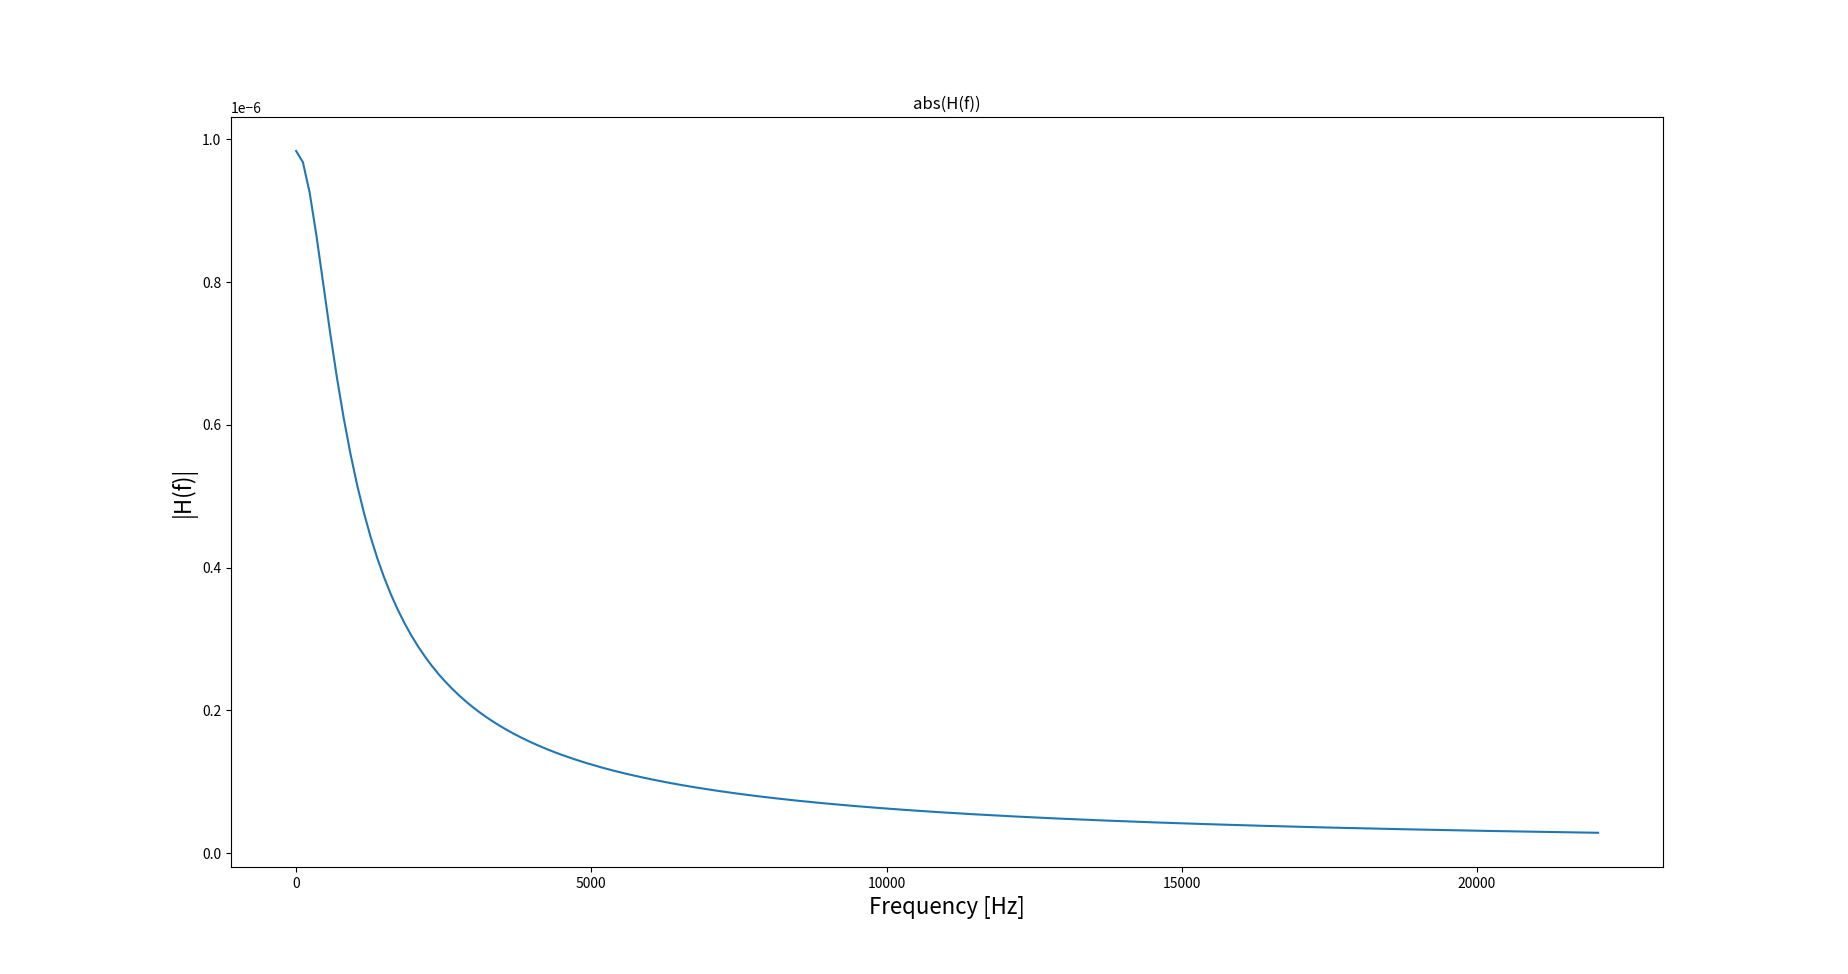
\includegraphics[width=160mm]{report/shortCircuitAtReceivingEndWithAttenuationConstant/frequencyTransferFunctionAbs.png}
    \caption{伝達関数}
    \label{p9}
  \end{center}
\end{figure}

\begin{figure}[H]
  \begin{center}
    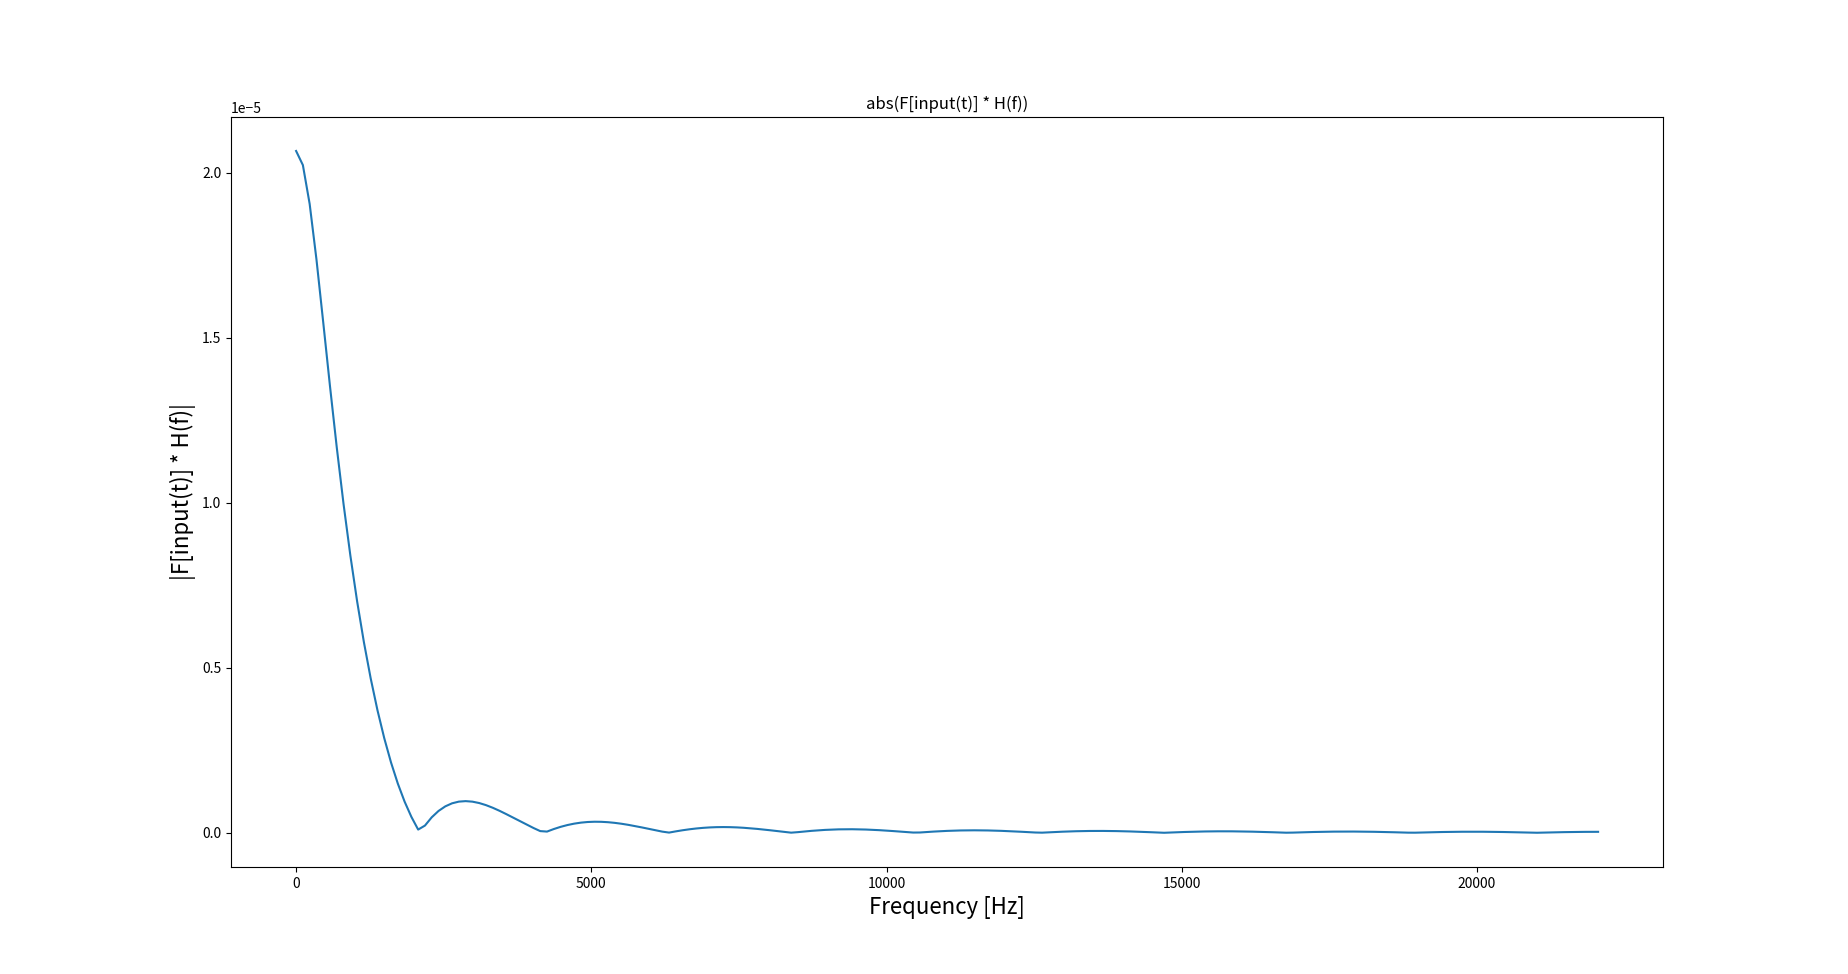
\includegraphics[width=160mm]{report/shortCircuitAtReceivingEndWithAttenuationConstant/productOfTFAndFTTOfInputWaveformAbs.png}
    \caption{伝達関数と入力波形をフーリエ変換したものの積}
    \label{p10}
  \end{center}
\end{figure}

\begin{figure}[H]
  \begin{center}
    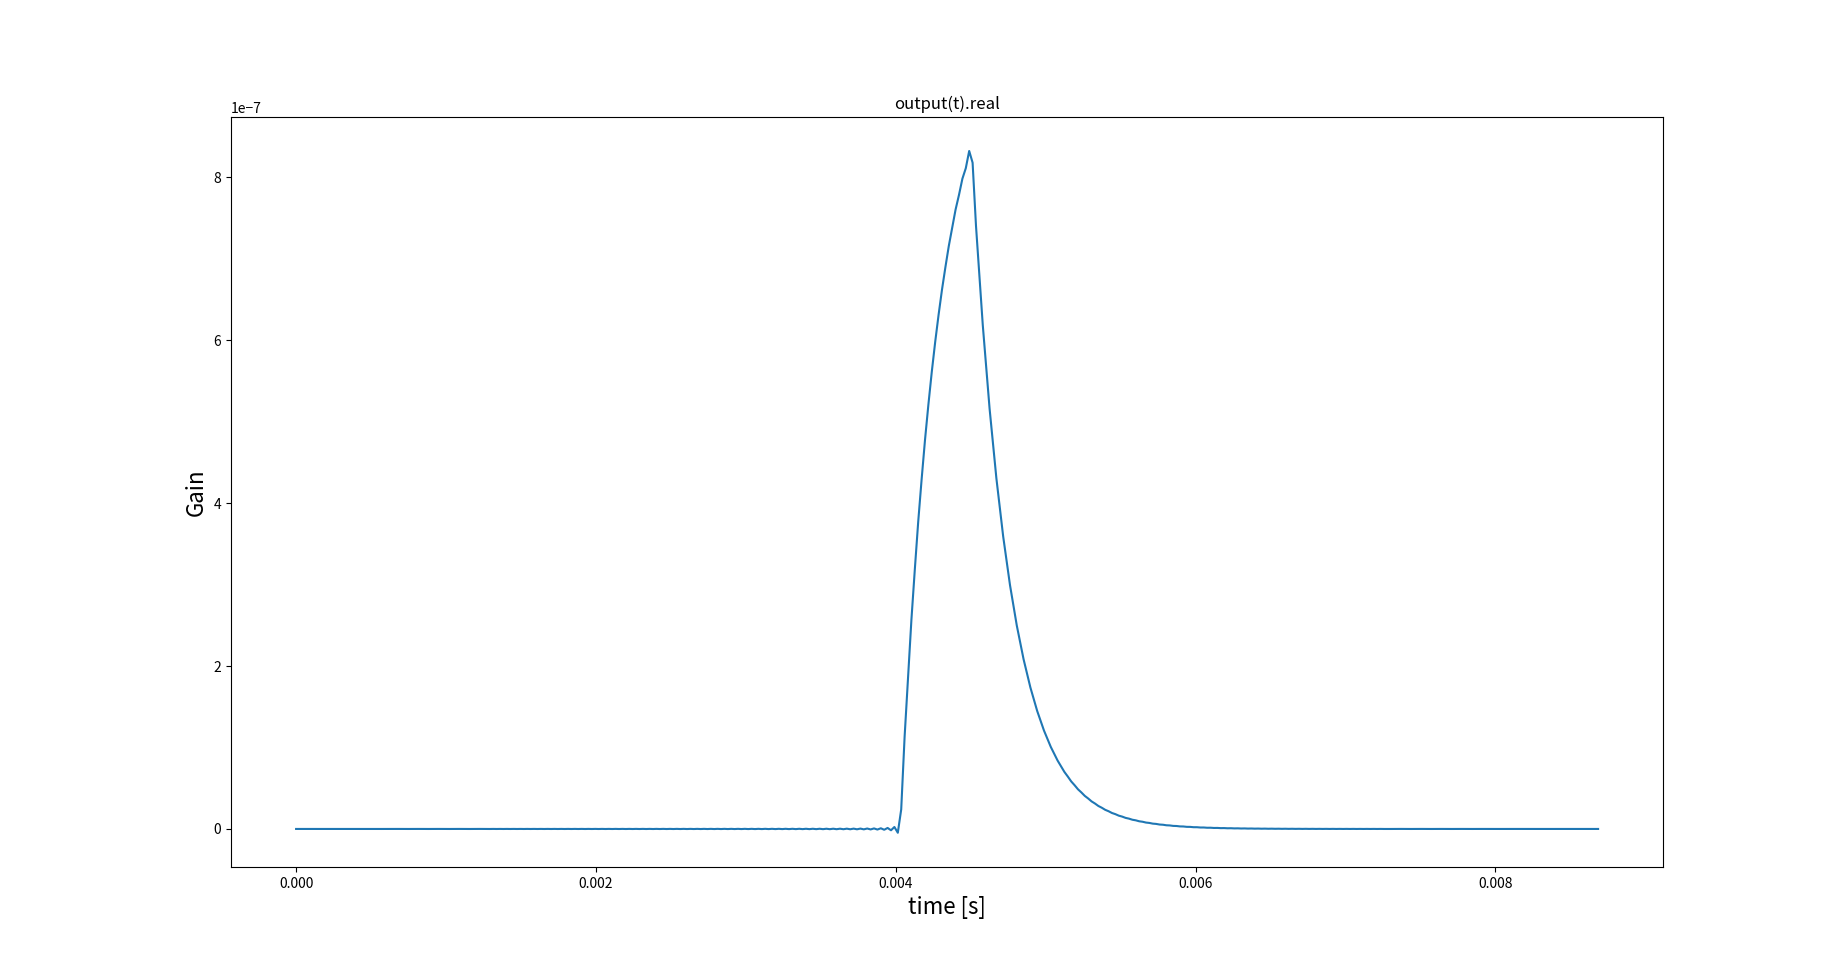
\includegraphics[width=160mm]{report/shortCircuitAtReceivingEndWithAttenuationConstant/outputWaveformTimeAxis.png}
    \caption{出力波形}
    \label{p11}
  \end{center}
\end{figure}

次に, 受電端を開放した場合の伝達関数, 伝達関数と入力波形をフーリエ変換したものの積, 伝達関数と入力波形をフーリエ変換したものの積を逆フーリエ変換して時間軸に戻した出力波形をそれぞれ図\ref{p12}, \ref{p13}, \ref{p14}に示す.

\begin{figure}[H]
  \begin{center}
    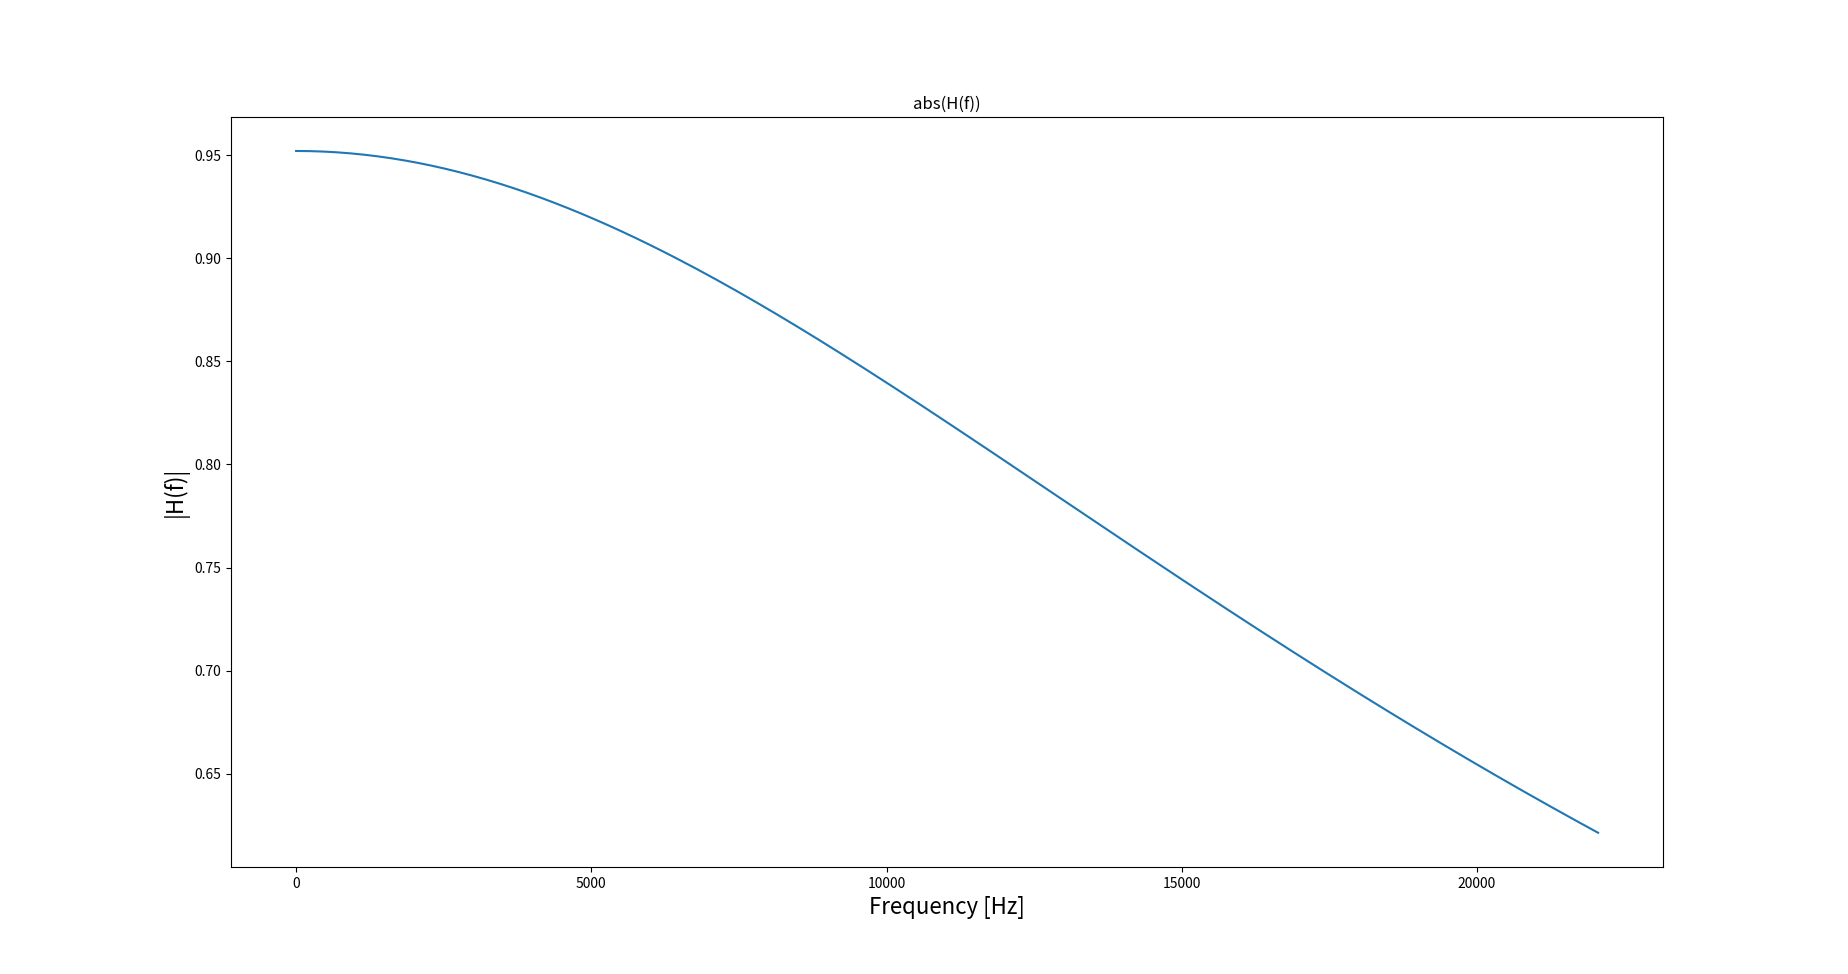
\includegraphics[width=160mm]{report/openAtReceivingEndWithAttenuationConstant/frequencyTransferFunctionAbs.png}
    \caption{伝達関数}
    \label{p12}
  \end{center}
\end{figure}

\begin{figure}[H]
  \begin{center}
    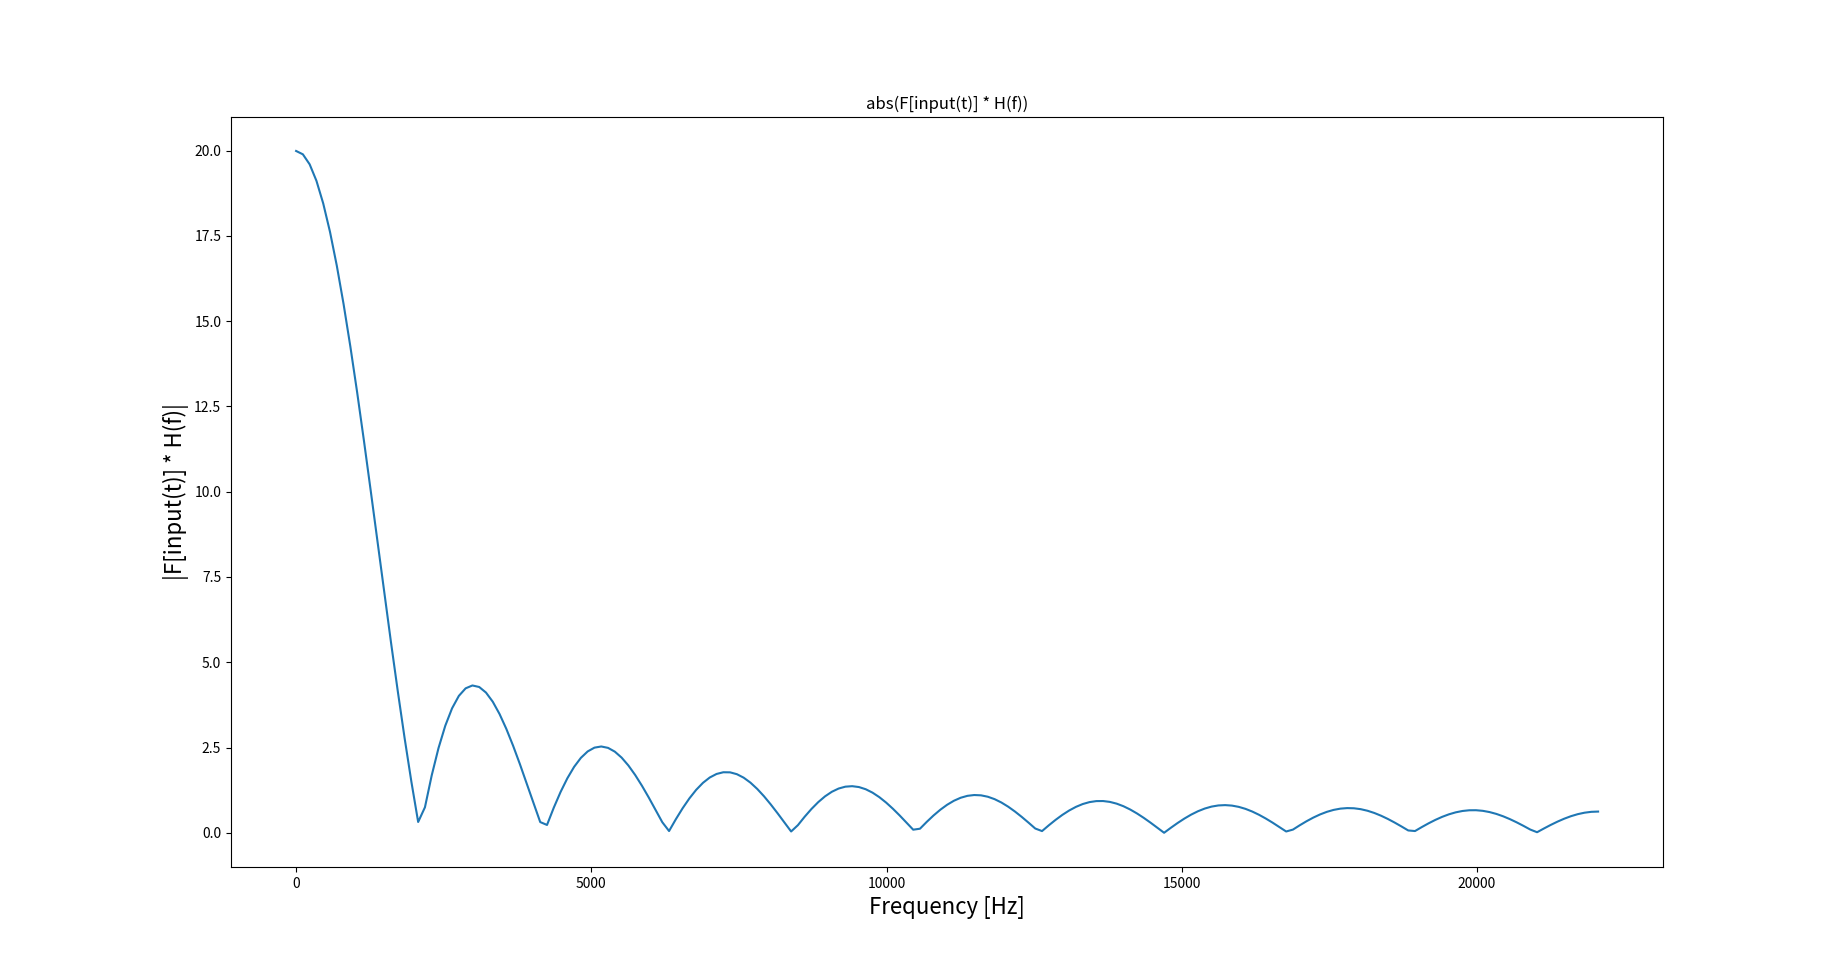
\includegraphics[width=160mm]{report/openAtReceivingEndWithAttenuationConstant/productOfTFAndFTTOfInputWaveformAbs.png}
    \caption{伝達関数と入力波形をフーリエ変換したものの積}
    \label{p13}
  \end{center}
\end{figure}

\begin{figure}[H]
  \begin{center}
    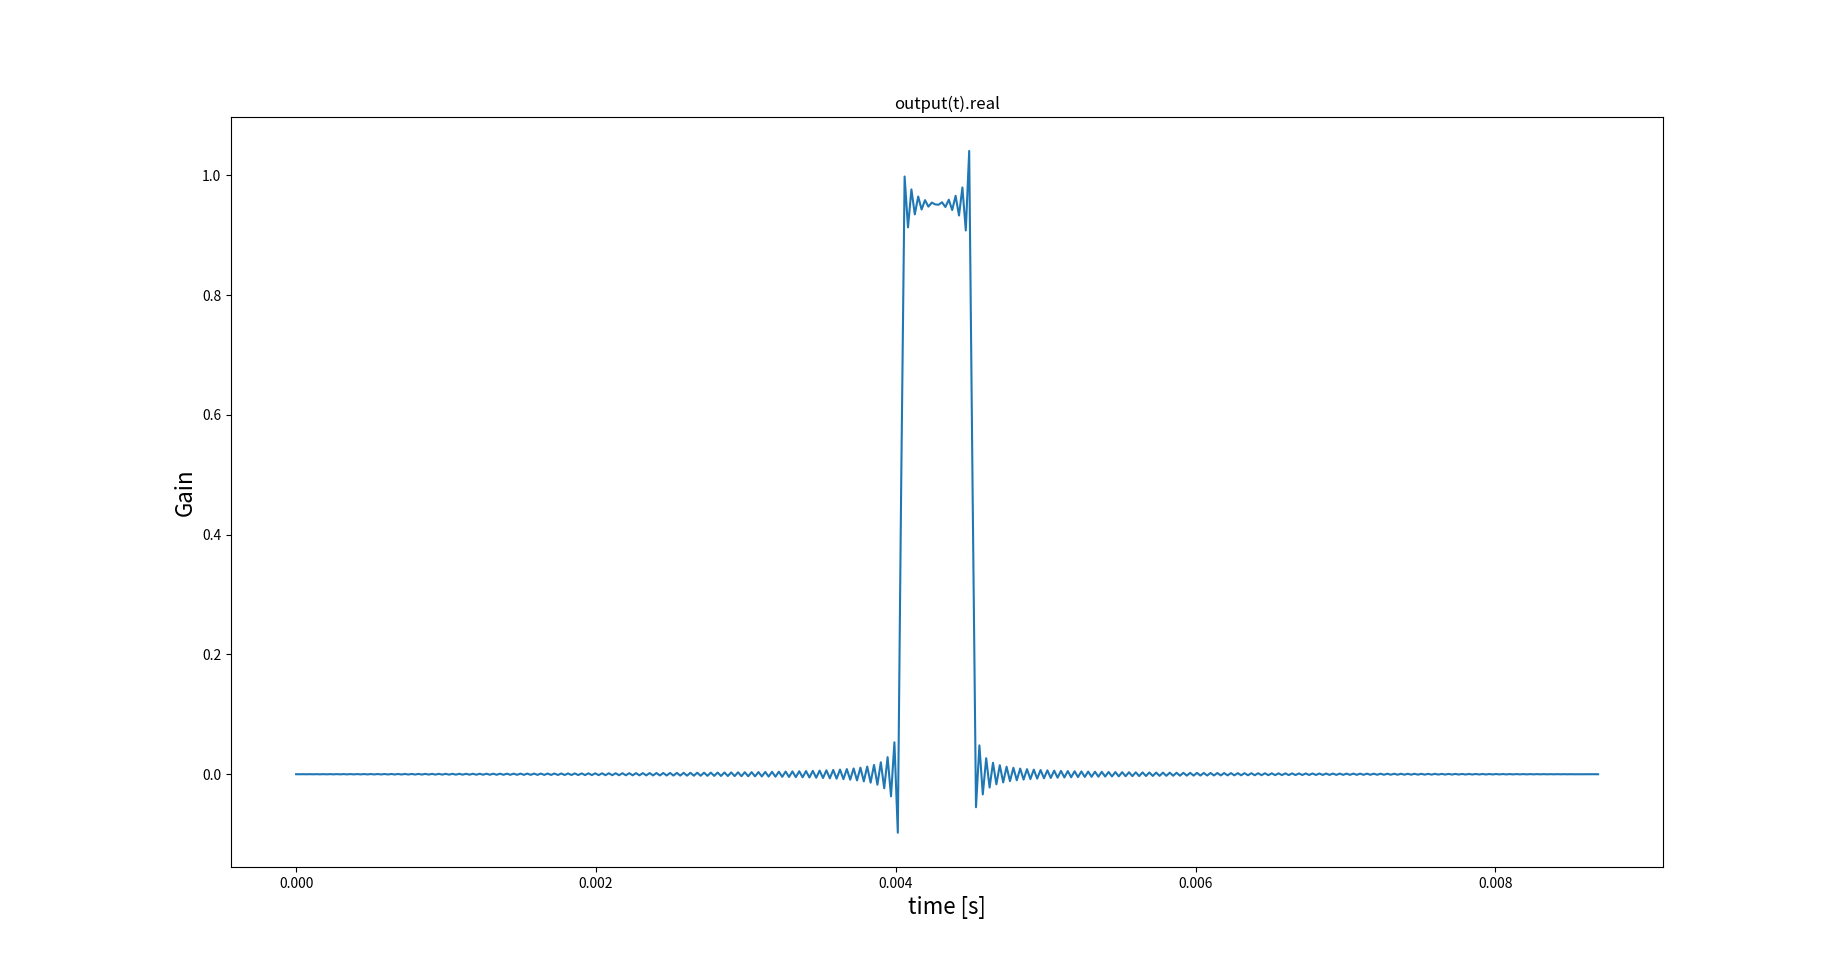
\includegraphics[width=160mm]{report/openAtReceivingEndWithAttenuationConstant/outputWaveformTimeAxis.png}
    \caption{出力波形}
    \label{p14}
  \end{center}
\end{figure}
\section{おわりに}

今回は, ケーブルをマッチング, もしくはマッチングせず受電端側を短絡, 開放した回路における周波数特性, 共振, 反共振について, また入力波形として方形波を入力した際の出力波形について調べた.

\begin{thebibliography}{5}
  \bibitem{1}大下 眞二郎,”詳解 電気回路演習 下”, 共立出版,参照 January 19,2022.
\end{thebibliography}

\end{document}